\csname documentclass\endcsname[../main.tex]{subfiles}
\usepackage[utf8x]{inputenc}
\usepackage{blindtext}
\usepackage{float}
\usepackage{graphicx}
\usepackage{siunitx}
\usepackage{cite}
\usepackage{hyperref}
\usepackage{cleveref}

% \DeclareSIUnit \bit {b}

\begin{document}

Co-developed by Massachusetts Institute of Technology (MIT), University of Florida (UF), and NASA's Ames Research Center (ARC), CLICK-A was launched to the International Space Station (ISS) on July 15th, 2022 at a \ang{51.6} inclination and \qty{414}{\kilo\meter} orbit. This section will take a look at the operations and results of the CLICK-A mission.

\subsection{System Overview}
As mentioned earlier, CLICK-A is a mission that will aim to verify technologies that will be used in the later CLICK-B/C missions. Since CLICK-A and CLICK-B/C share components, in-space operation experience will provide more confidence for the later mission.
The CLICK-A and CLICK-B/C terminals share a few components, namely the microelectromechanical systems (MEMS), a silicon CMOS camera, an Erbium-doped fiber amplifier, and a fine steering motor \cite{click_a}.

The optical communications terminal for CLICK-A was designed to transmit at rates ranging between 5-50 \unit[per-mode = symbol,per-symbol = p]{\mega\bit\per\second}.

\begin{figure*}[t]
    \centering
    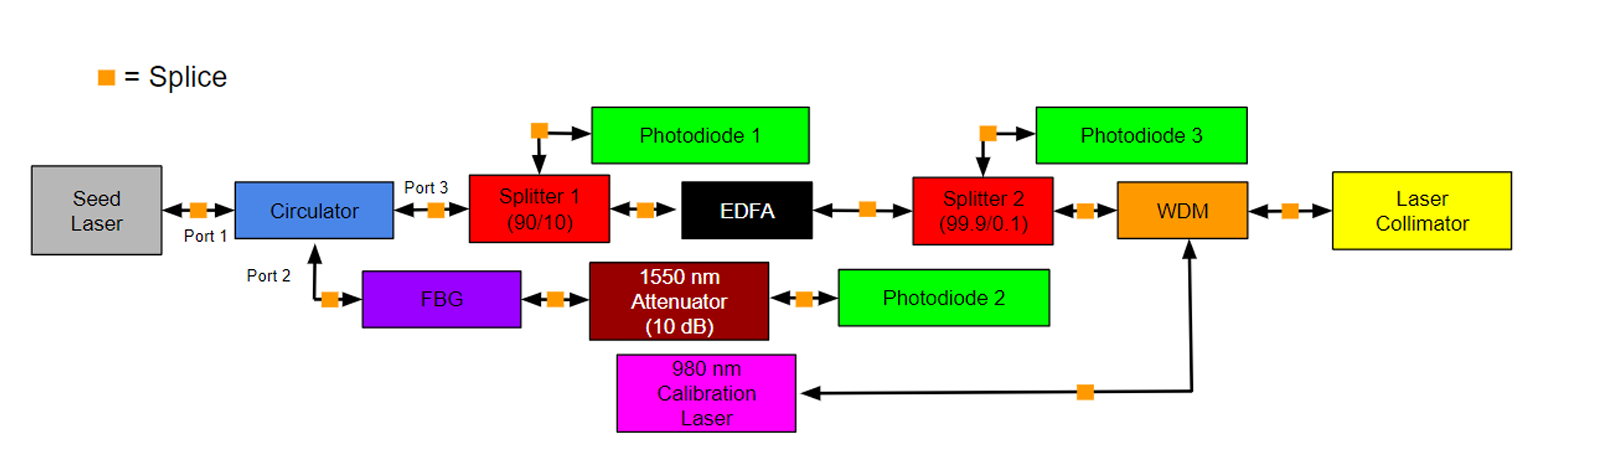
\includegraphics[width=\textwidth, height=200pt]{images/click_a_fiber_comp.PNG}
    \caption{Fiber Optic assembly of the CLICK-A terminal \cite{click_a}.}
    \label{fig:fiber_optic}
\end{figure*}

\begin{figure}[H]
    \centering
    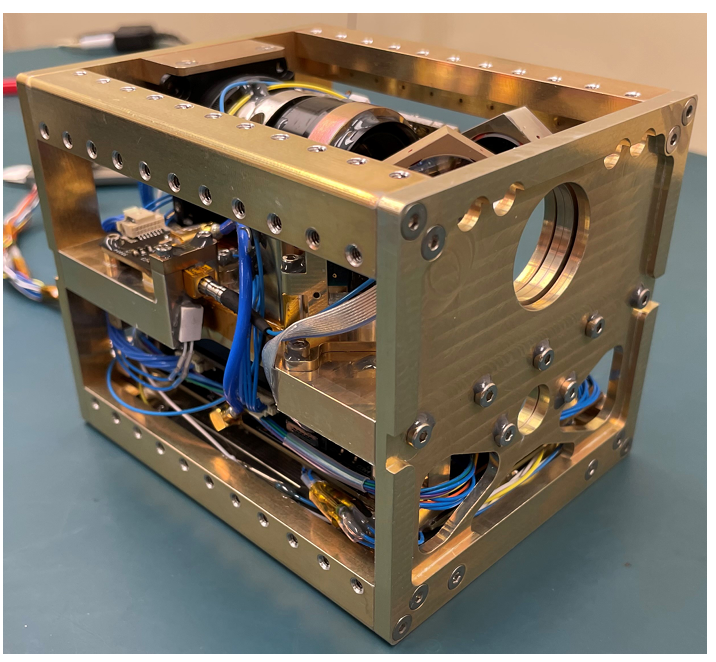
\includegraphics[width=200pt, height=200pt]{images/click_a_flight_model.PNG}
    \caption{CLICK-A terminal flight model \cite{click_a}.}
    \label{fig:flight_model_a}
\end{figure}

The flight model terminal, shown in \Cref{fig:flight_model_a}, is paired with a low-cost optical ground stations (OGS), which is based on a telescope with additional backend optics and receivers to allow for optical communications.

\subsection{The Terminal}

The terminal for CLICK-A uses a \(\qty{5}{\nano\second}\) slot width pulse position modulation (PPM). In order to handle the power scaling of the laser, CLICK-A utilizes the popular master oscillator power amplifier (MOPA) approach. \Cref{fig:fiber_optic} shows the fiber components for the terminal itself. The terminal has many components such as \cite{click_a}:
\begin{itemize}
    \item Athermal Fiber Bragg Grating (FBG)
    \item \qty{200}{\milli\watt} Erbium Doped Fiber Amplifier
    \item Collimator
\end{itemize}

The design allows the terminal to control the fine pointing of the transmitting beam independently while also being able to reject most of the mispointing caused by the spacecraft's body pointing \cite{click_a}.

\subsection{The Optical Downlink}

There was regular communications with the CLICK-A spacecraft for health telemtery and for troubleshooting any issues since the last contact.
The most important piece of data was the GPS data gained from the telemetry data since it was instrumental in ascertaining the errors between the spacecrafts actual and projected position \cite{click_a}. 

In order to have a successful contact, the spacecrafts orbit was mapped out weeks ahead to better know when it would pass over the OGS.
To even select passes as successful downlink candidates, the orbit was cross-referenced with clear weather and a minimum elevation angle of \ang{40}.
The weather plays a part since optical frequencies are prone to attenuation caused by the water vapor, so clear weather was preferred \cite{click_a}. 

In order to test the precision pointing of the OGS, the most recent NORAD TLE set is enhanced with SGP4 batch least squares orbit fit to the most up-to-date GPS data. 
This allowed for the prediciton of where the spacecraft would be along the orbital path to be used in the precision pointing of the ground station \cite{click_a}.

In order to have a successful downlink, the spacecraft would first need to "see" the beacon on the OGS. Once the satellite terminal has verified the beacon, the controller drives its mirror to an angle that can successfully direct the transmit laser to the OGS \cite{click_a}. Once the OGS is able to see the laser it can better position itself to better point the beacon laser \cite{click_a}.

\begin{figure*}[t]
    \centering
    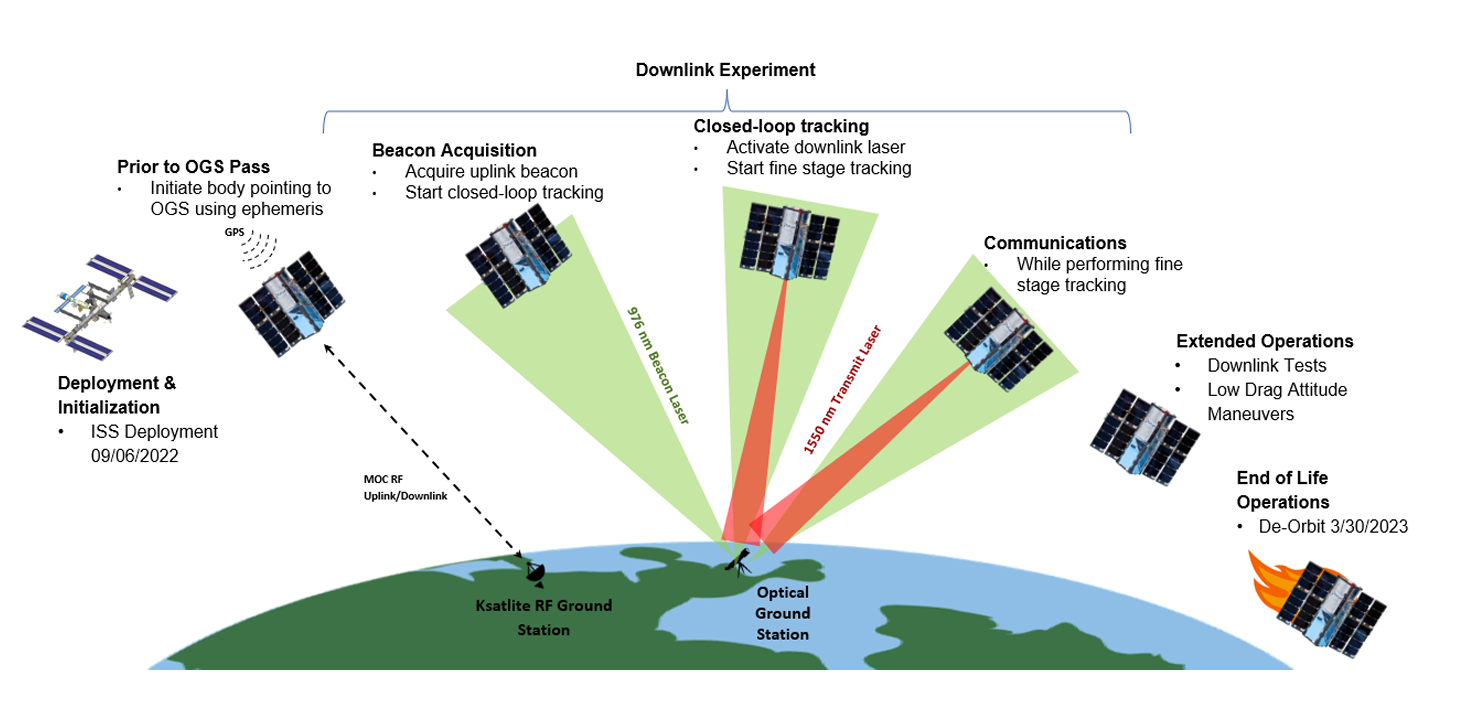
\includegraphics[width=\textwidth, height=200pt]{images/click_a_downlink.PNG}
    \caption{Concept of Operations for the CLICK-A mission \cite{click_a}.}
    \label{fig:conops}
\end{figure*}

The concept of operations for the CLICK-A mission is shown in \Cref{fig:conops}.



\end{document}